\documentclass[a4paper,12pt]{article}
\usepackage[top=2.5cm, bottom=2.5cm, left=2.5cm, right=2.5cm]{geometry}
\usepackage[utf8x]{inputenc}
\usepackage[T1]{fontenc}
\usepackage[french]{babel} 
\usepackage{hyperref}
\usepackage{graphicx}
\usepackage{url}
\makeatletter
\g@addto@macro{\UrlBreaks}{\UrlOrds}
\makeatother

\author{\textsc{Jorandon} Guillaume}
\date{22 mai 2017} 
\title{Fiche de lecture\\\large{\textit{Google’s autocompletion: algorithms, stereotypes and accountability}}\\\normalsize{SC22}}


\begin{document}

\maketitle

Source : \url{http://sociostrategy.com/2013/googles-autocompletion-algorithms-stereotypes-accountability/}\\

Il s'agit d'un article de 2013 publié sur \url{sociostrategy.com}, le blog de Anna \textsc{Jobin}, doctorante en sociologie du Laboratoire de cultures et humanités digitales de l'Université de Lausanne, en Suisse. L'article cherche à questionner la responsabilité de Google dans les dérives observées à propos de l'algorithme d'autocomplétion de son moteur de recherche phare.

L'article commence par une illustration de xkcd\footnote{Il est à noter que xkcd, webcomic à l'initiative de Randall \textsc{Munroe} (un ancien de la NASA), aborde régulièrement d'une plume acerbe et satirique des thèmes liés à une approche culturelle des technologies numériques : linguistique, sociologie, politique, mathématiques...} à propos de l'autocomplétion parfois incongrue des grandes question existentielles que peuvent poser les utilisateur-ice-s de Google. N'importe qui pourra d'ailleurs vérifier cela en écrivant "Why" sur Google (figure \ref{why}).

\begin{figure}[ht]
 \begin{center}
  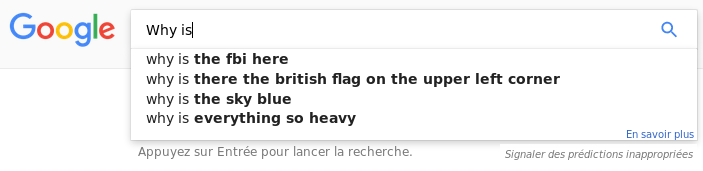
\includegraphics[width=150px]{why.png}
 \end{center}
 \caption{Why is the FBI here?}
 \label{why}
\end{figure}

Cependant, et comme l'article le montre par la suite, cette amusante autocomplétion prend une dimension beaucoup plus perturbante dès que l'on commence à chercher des réponses à des questions sur "les femmes." \textsc{Jobin} illustre cela avec des affiches de \textit{The autocomplete Truth}, une campagne de l'ONU sur les droits des femmes qui met en lumière les stéréotypes véhiculés par l'autocomplétion de Google (figure \ref{campagne}). Si cette campagne a été un succès (figure \ref{succes}), il faut toutefois noter, comme le relève Anna \textsc{Jobin}, qu'une majorité des gens s'est contentée de constater l'existence de ces résultats dans les suggestions de recherche du moteur, sans les problématiser ni les mettre en parallèle avec la problématique globale du sexisme.

\begin{figure}[ht]
 \begin{center}
  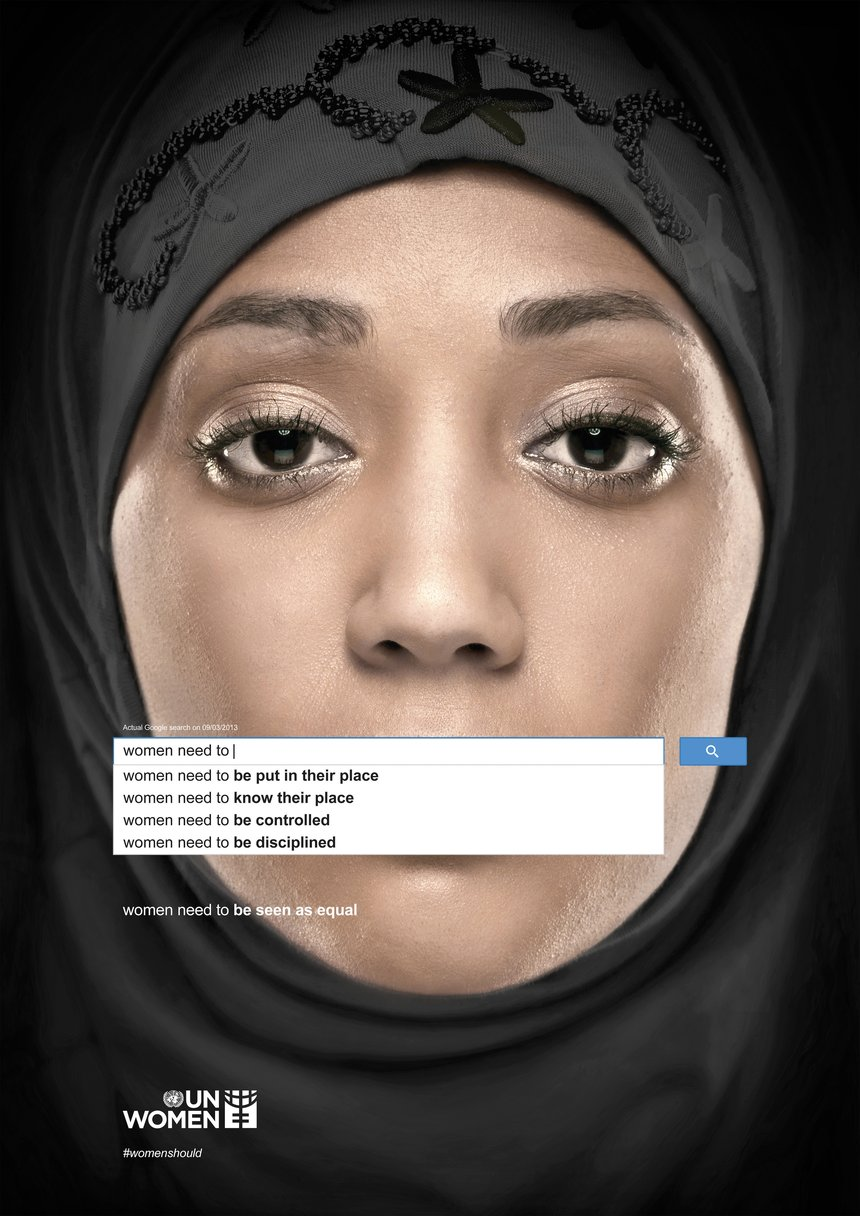
\includegraphics[width=150px]{campagne.jpg}
 \end{center}
 \caption{Extrait de la campagne \textit{The Autocomplete Truth} de l'ONU.}
 \label{campagne}
\end{figure}

\begin{figure}[ht]
 \begin{center}
  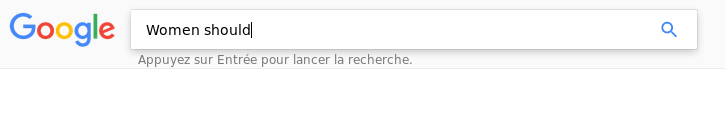
\includegraphics[width=150px]{success.png}
 \end{center}
 \caption{Google a d'ailleurs supprimé les suggestions de recherche incriminées.}
 \label{succes}
\end{figure}

L'autrice revient ensuite sur ses recherches à propos des algorithmes d'autocomplétion de Google, à travers un article qu'elle a co-signé avec Frédéric \textsc{Kaplan}, chaire de \textit{Digital Humanities} et directeur du laboratoire DHLab à Lausanne. Elle y explique notamment pourquoi ce mécanisme d'autocomplétion est une prothèse linguistique, c'est à dire qu'il est un relai entre la pensée et son expression écrite. Par sa suggestion a posteriori (l'autocomplétion intervient avant que l'utilisateur-ice ait terminé de saisir sa requête), l'autocomplétion peut accidentellement induire des recherches qu'une personne n'aurait pas cherché à la base et, dans le contexte qui nous intéresse, se faire le relai de stéréotypes négatifs. Ainsi, par effet de cercle vicieux, la présence de ces suggestions renforce les mécanismes d'oppressions, et ces mécanismes d'oppression augmentent les occurrences de ces suggestions stéréotypées. Ce mécanisme d'auto-renforcement est aussi à la base du concept de bulle de filtres, que l'on observe notamment sur Facebook \footnote{Jeff \textsc{Yates} a testé concrètement cet effet. \url{http://ici.radio-canada.ca/nouvelle/1029916/experience-facebook-algorithmes-bulle-desinformation?fromBeta=true}}, et qui peut induire un biais de confirmation \footnote{\url{http://www.sceptiques.qc.ca/dictionnaire/confirmbias.html}} énorme. Dans un autre registre, cet effet de cercle a pu s'observer quand \textit{Tay}, une intelligence artificielle conversationnelle mise sur Twitter à disposition du public par Microsoft, est devenu vulgaire et antisémite sous l'influence des conversations avec des trolls de l'\textit{alt-right}\footnote{\url{http://www.telegraph.co.uk/technology/2016/03/24/microsofts-teen-girl-ai-turns-into-a-hitler-loving-sex-robot-wit/}}.

Sur qui donc jeter l'oprobe ? Google affirme que son moteur de recherche est le reflet objectif de ce que veulent chercher les gens. Mais il ne faut pas oublier que Google reste une entreprise américaine à but lucratif, qui peut pratiquer une censure privée sur les résultats et les suggestions de recherche : pour des raisons purement commerciales certes, mais parfois aussi morales ou légales. Loins d'être objectives, les suggestions de recherche sont avant tout un reflet plus ou moins direct des modes de pensée de ses utilisateur-ice-s et concepteur-ice-s.

Il serait cependant précipité d'attribuer à Google l'entière responsabilité de ces dérives. L'autrice suggère notamment le rôle des activistes méninistes et virilistes, qui opèrent un retour en force ces dernières années grâce à Internet et les réseaux sociaux. Cette mouvance souvent proche de l'extrême-droite se développe en réaction à une supposée "crise de la masculinité", et prône un retour à des valeurs patriarcales traditionnelles plaçant un sexe masculin fort comme pilier de la société. Ou placer alors la responsabilité ? En dépit de la posture cynique affichée par Google, ses algorithmes ne sont pas neutres et objectifs. Un algorithme qui sélectionne et analyse l'information, et qui prend une décision sur la base de cette analyse, ne peut le faire sur des critères entièrement objectifs. 

Ainsi, la question de la responsabilité des algorithmes sur les dérives que nous venons d'observer est très complexe, car elle est fonction d'énormément de facteurs. Google n'est ni complètement coupable, ni entièrement innocent, et il convient de se demander à qui attribuer les responsabilités que l'on délègue aux algorithmes.

\end{document}
